\documentclass[aspectratio=169,10pt]{ctexbeamer}

\usetheme{Madrid}
\usecolortheme{default}

\usepackage{amsmath,amssymb,mathtools,bm}
\usepackage{tikz}
\usetikzlibrary{arrows.meta,calc,positioning}

\makeatletter
\def\input@path{{../模板/}}
\makeatother
\usepackage{yingxing-beamer}

\definecolor{MainBlue}{RGB}{25,70,140}
\definecolor{AccentRed}{RGB}{180,60,45}
\definecolor{SoftBg}{RGB}{246,248,252}
\setbeamercolor{alerted text}{fg=AccentRed}

\newcommand{\R}{\mathbb{R}}
\newcommand{\dd}{\,\mathrm{d}}
\newcommand{\ee}{\mathrm{e}}
\newcommand{\ii}{\mathrm{i}}

\title{积分计算、微分方程与极值}
\subtitle{}
\author{}
\date{}

\begin{document}

\begin{frame}
  \titlepage
\end{frame}

\begin{frame}{本次内容}
\small
\tableofcontents
\end{frame}

\begin{frame}[t]{整体主线}
\small
\begin{block}{积分计算}
核心不是背单个公式，而是把被积函数归入可处理的类型：
\[
\text{原函数与不定积分}\quad
\text{换元积分}\quad
\text{分部积分}\quad
\text{有理函数}\quad
\text{有理三角函数}\quad
\text{可有理化的无理函数}.
\]
\end{block}

\begin{block}{极值问题}
后半部分从“导数为零”出发，研究
\[
\text{极值点}\quad
\text{最值点}\quad
\text{驻点}.
\]
\end{block}

\begin{block}{微分方程}
求原函数可以看作求解最简单的微分方程：
\[
  F'=f.
\]
在此基础上引入微分算子、齐次方程、非齐次方程和常数变易法。
\end{block}
\end{frame}

\section{原函数与不定积分}

\begin{frame}[t]{从导数反推函数}
\small
\begin{block}{基本问题}
给定函数 $f$，寻找可微函数 $F$，使得
\[
  F'(x)=f(x).
\]
这样的 $F$ 称为 $f$ 的一个原函数。
\end{block}

\begin{block}{唯一性到常数为止}
如果 $F_1'(x)=f(x)$，$F_2'(x)=f(x)$，则
\[
  (F_1-F_2)'=0.
\]
因此在同一区间上
\[
  F_1(x)-F_2(x)=C.
\]
也就是说，同一个函数的任意两个原函数只差一个常数。
\end{block}
\end{frame}

\begin{frame}[t]{不定积分的记号}
\small
\begin{block}{定义}
若 $F$ 是 $f$ 在区间 $I$ 上的一个原函数，则记
\[
  \int f(x)\,\dd x=F(x)+C,\qquad x\in I.
\]
这里 $C$ 为任意常数。
\end{block}

\begin{block}{理解}
不定积分不是单个函数，而是一族函数：
\[
  \{F(x)+C:C\in\R\}.
\]
求不定积分，本质上就是求微分运算的逆运算：
\[
  \dd F=f(x)\dd x,\qquad
  \dd\!\left(\int f(x)\dd x\right)=f(x)\dd x.
\]
\end{block}
\end{frame}

\begin{frame}[t]{基本不定积分公式（一）}
\small
\begin{block}{代数与指数}
\[
\begin{array}{rlrl}
\displaystyle \int 0\,\dd x&=C,&
\displaystyle \int x^\alpha\,\dd x&=\frac{x^{\alpha+1}}{\alpha+1}+C\quad(\alpha\ne-1),\\[2mm]
\displaystyle \int\frac{\dd x}{x}&=\ln|x|+C,&
\displaystyle \int \ee^x\,\dd x&=\ee^x+C,\\[2mm]
\displaystyle \int a^x\,\dd x&=\frac{a^x}{\ln a}+C\quad(a>0,\ a\ne1),&
\displaystyle \int\frac{\dd x}{1+x^2}&=\arctan x+C.
\end{array}
\]
\end{block}

\begin{block}{使用方式}
这些公式都来自对应的求导公式。例如
\[
  \left(\frac{x^{\alpha+1}}{\alpha+1}\right)'=x^\alpha,\qquad
  (\ln|x|)'=\frac1x.
\]
\end{block}
\end{frame}

\begin{frame}[t]{基本不定积分公式（二）}
\small
\begin{block}{三角与反三角}
\[
\begin{array}{rlrl}
\displaystyle \int\cos x\,\dd x&=\sin x+C,&
\displaystyle \int\sin x\,\dd x&=-\cos x+C,\\[2mm]
\displaystyle \int\sec^2x\,\dd x&=\tan x+C,&
\displaystyle \int\csc^2x\,\dd x&=-\cot x+C,\\[2mm]
\displaystyle \int\frac{\dd x}{\sqrt{1-x^2}}&=\arcsin x+C,&
\displaystyle \int\frac{\dd x}{1+x^2}&=\arctan x+C.
\end{array}
\]
\end{block}

\begin{block}{含根式的常用公式}
\[
  \int\frac{\dd x}{\sqrt{1+x^2}}
  =\ln\!\left(x+\sqrt{1+x^2}\right)+C.
\]
\end{block}
\end{frame}

\begin{frame}[t]{Newton--Leibniz 公式}
\small
\begin{block}{连续函数一定有原函数}
若 $f$ 在区间 $I$ 上连续，$a\in I$，则
\[
  F(x)=\int_a^x f(t)\,\dd t
\]
是 $f$ 的一个原函数，即
\[
  F'(x)=f(x).
\]
\end{block}

\begin{block}{定积分计算公式}
若 $F'(x)=f(x)$，则
\[
  \int_a^b f(x)\,\dd x
  =F(b)-F(a)
  =F(x)\bigg|_a^b.
\]
这说明：先求不定积分，再代入上下限，就可以计算相应的定积分。
\end{block}
\end{frame}

\begin{frame}[t]{不定积分的线性性质}
\small
\begin{block}{公式}
若 $f,g$ 在同一区间上都有原函数，则对任意常数 $\alpha,\beta$，
\[
  \int \bigl(\alpha f(x)+\beta g(x)\bigr)\,\dd x
  =\alpha\int f(x)\,\dd x+\beta\int g(x)\,\dd x.
\]
\end{block}

\begin{block}{使用方式}
线性性质允许我们先拆项，再分别积分：
\[
  \int \left(3x^2+1\right)\dd x
  =3\int x^2\,\dd x+\int 1\,\dd x
  =x^3+x+C.
\]
这也是后面有理函数积分中“先分解，再积分”的基础。
\end{block}
\end{frame}

\begin{frame}[t]{基本计算：直接套公式}
\small
\begin{block}{题目}
求
\[
  \int\left(x+\frac1{\sqrt{x}}\right)\dd x,\qquad x>0.
\]
\end{block}

由线性性质与幂函数公式，
\[
\begin{aligned}
\int\left(x+\frac1{\sqrt{x}}\right)\dd x
&=\int x\,\dd x+\int x^{-1/2}\,\dd x\\
&=\frac{x^2}{2}+2\sqrt{x}+C.
\end{aligned}
\]

\begin{alertblock}{注意}
不定积分结果中的常数统一写成一个 $C$，不必给每一项分别写常数。
\end{alertblock}
\end{frame}

\begin{frame}[t]{基本计算：先裂项}
\small
\begin{block}{题目}
设 $a\ne0$，求
\[
  \int\frac{\dd x}{x^2-a^2}.
\]
\end{block}

先分解：
\[
  \frac1{x^2-a^2}
  =\frac1{(x-a)(x+a)}
  =\frac1{2a}\left(\frac1{x-a}-\frac1{x+a}\right).
\]
于是
\[
\begin{aligned}
\int\frac{\dd x}{x^2-a^2}
&=\frac1{2a}\left(\ln|x-a|-\ln|x+a|\right)+C\\
&=\frac1{2a}\ln\left|\frac{x-a}{x+a}\right|+C.
\end{aligned}
\]
\end{frame}

\section{换元积分法}

\begin{frame}[t]{换元积分法：作用}
\small
\begin{block}{核心目标}
把不容易直接求原函数的积分，改写成另一个变量下更熟悉的积分：
\[
  \int f(\varphi(x))\varphi'(x)\,\dd x
  \quad\longrightarrow\quad
  \int f(u)\,\dd u.
\]
\end{block}

\begin{block}{两种常用形式}
\[
\begin{array}{ll}
\text{第一类换元} & u=\varphi(x),\quad \dd u=\varphi'(x)\dd x,\\[2mm]
\text{第二类换元} & x=\psi(t),\quad \dd x=\psi'(t)\dd t.
\end{array}
\]
第一类常用于“凑微分”，第二类常用于根式、三角式或区间端点更自然的情形。
\end{block}
\end{frame}

\begin{frame}[t]{第一类换元：凑微分}
\small
\begin{block}{不定积分公式}
设 $F'(u)=f(u)$，$u=\varphi(x)$ 可微，则
\[
  \int f(\varphi(x))\varphi'(x)\,\dd x
  =F(\varphi(x))+C.
\]
记号上可写成
\[
  \int f(u)\,\dd u=F(u)+C,\qquad u=\varphi(x).
\]
\end{block}

\begin{block}{使用判断}
如果被积式中同时出现“复合函数”和“内层函数的导数”，通常优先尝试第一类换元。
\[
  f(\varphi(x))\varphi'(x)\,\dd x
  \quad\leadsto\quad
  f(u)\,\dd u.
\]
\end{block}
\end{frame}

\begin{frame}[t]{第一类换元：两个基本例子}
\small
\begin{block}{三角函数中的凑微分}
\[
\begin{aligned}
\int \cot x\,\dd x
&=\int \frac{\cos x}{\sin x}\,\dd x.
\end{aligned}
\]
令 $u=\sin x$，则 $\dd u=\cos x\,\dd x$，故
\[
  \int \cot x\,\dd x
  =\int \frac{\dd u}{u}
  =\ln|u|+C=\ln|\sin x|+C.
\]
\end{block}

\begin{block}{指数函数中的凑微分}
\[
\begin{aligned}
\int\frac{\dd x}{1+\ee^x}
&=\int\frac{\ee^{-x}}{1+\ee^{-x}}\,\dd x.
\end{aligned}
\]
令 $u=\ee^{-x}$，则 $\dd u=-\ee^{-x}\dd x$，所以
\[
  \int\frac{\dd x}{1+\ee^x}
  =-\int\frac{\dd u}{1+u}
  =-\ln(1+\ee^{-x})+C.
\]
\end{block}
\end{frame}

\begin{frame}[t]{定积分换元：上下限同步替换}
\small
\begin{block}{公式}
若 $u=\varphi(x)$，$\varphi$ 连续可微，则
\[
  \int_a^b f(\varphi(x))\varphi'(x)\,\dd x
  =\int_{\varphi(a)}^{\varphi(b)} f(u)\,\dd u.
\]
定积分换元时，换变量以后应同时换上下限；这样计算过程中不必再回代。
\end{block}

\begin{block}{例}
求
\[
  \int_0^2 x\ee^{x^2}\,\dd x.
\]
令 $u=x^2$，则 $\dd u=2x\dd x$，且 $x=0,2$ 时 $u=0,4$，所以
\[
  \int_0^2 x\ee^{x^2}\,\dd x
  =\frac12\int_0^4\ee^u\,\dd u
  =\frac{\ee^4-1}{2}.
\]
\end{block}
\end{frame}

\begin{frame}[t]{第二类换元：换掉原变量}
\small
\begin{block}{不定积分公式}
令 $x=\psi(t)$，其中 $\psi$ 在所讨论区间内可微且可逆。若
\[
  \int f(\psi(t))\psi'(t)\,\dd t=G(t)+C,
\]
则
\[
  \int f(x)\,\dd x=G(\psi^{-1}(x))+C.
\]
\end{block}

\begin{block}{定积分形式}
若 $\psi(\alpha)=a,\ \psi(\beta)=b$，则
\[
  \int_a^b f(x)\,\dd x
  =\int_\alpha^\beta f(\psi(t))\psi'(t)\,\dd t.
\]
根式积分中常令 $x=a\sin t$、$x=a\tan t$、$x=a\sec t$，本质都是第二类换元。
\end{block}
\end{frame}

\begin{frame}[t]{例 1：三角换元处理定积分}
\small
\begin{block}{例 1}
求
\[
  \int_0^a \sqrt{a^2-x^2}\,\dd x,\qquad a>0.
\]
\end{block}

令 $x=a\sin t,\ t\in[0,\pi/2]$，则
\[
\begin{aligned}
\int_0^a \sqrt{a^2-x^2}\,\dd x
&=\int_0^{\pi/2} a\cos t\cdot a\cos t\,\dd t  \\
&=\frac{a^2}{2}\int_0^{\pi/2}(1+\cos 2t)\,\dd t
=\frac{\pi a^2}{4}.
\end{aligned}
\]
\end{frame}

\begin{frame}[t]{换元选择：常见信号}
\small
\begin{block}{第一类换元优先}
\[
\begin{array}{ll}
g'(x)\,f(g(x)) & \text{令 } u=g(x),\\[1mm]
\frac{g'(x)}{g(x)} & \text{令 } u=g(x),\\[1mm]
\ee^{g(x)}g'(x),\ \sin g(x)g'(x) & \text{令 } u=g(x).
\end{array}
\]
\end{block}

\begin{block}{第二类换元优先}
\[
\begin{array}{ll}
\sqrt{a^2-x^2} & x=a\sin t,\\[1mm]
\sqrt{a^2+x^2} & x=a\tan t,\\[1mm]
\sqrt{x^2-a^2} & x=a\sec t\quad (x\ge a).
\end{array}
\]
选择代换的标准不是形式漂亮，而是代换后被积函数是否更接近基本积分、有理函数积分或三角恒等式。
\end{block}
\end{frame}

\section{分部积分法}

\begin{frame}[t]{命题 1：分部积分法}
\small
\begin{block}{不定积分形式}
设 $u(x),v(x)$ 在区间 $I$ 中可微。若 $u'(x)v(x)$ 有原函数，则 $u(x)v'(x)$ 也有原函数，且
\[
  \int u(x)v'(x)\,\dd x
  =u(x)v(x)-\int u'(x)v(x)\,\dd x.
\]
\end{block}

\begin{block}{微分形式}
\[
  \int u\,\dd v=uv-\int v\,\dd u.
\]
\end{block}

\begin{block}{定积分形式}
若 $u,v$ 连续可微，则
\[
  \int_a^b u(x)v'(x)\,\dd x
  =u(x)v(x)\bigg|_a^b-\int_a^b u'(x)v(x)\,\dd x.
\]
\end{block}
\end{frame}

\begin{frame}[t]{分部积分法：证明}
\small
由乘积求导公式
\[
  [u(x)v(x)]'=u'(x)v(x)+u(x)v'(x),
\]
得
\[
  \left[u(x)v(x)-\int u'(x)v(x)\,\dd x\right]'=u(x)v'(x).
\]

\vspace{0.5em}
因此
\[
  u(x)v(x)-\int u'(x)v(x)\,\dd x
\]
是 $u(x)v'(x)$ 的原函数，命题成立。
\end{frame}

\begin{frame}[t]{分部积分法：概念和选取原则}
\small
\begin{block}{核心思想}
把一个“不方便直接积分”的乘积，改写成另一个更容易积分的乘积：
\[
  \int u\,\dd v=uv-\int v\,\dd u.
\]
关键在于让 $\dd u$ 变简单，或让 $v$ 可明确写出。
\end{block}

\begin{block}{常见选择}
\begin{itemize}
  \item 含 $\ln x$ 或反三角函数：通常令它作 $u$，求导后复杂度下降；
  \item 多项式乘三角/指数函数：通常令多项式作 $u$，反复分部可降低幂次；
  \item 积分式两边同时出现原积分：移项后得到结果；
  \item 三角幂、分母含参数的积分：常通过分部积分建立递推公式。
\end{itemize}
\end{block}
\end{frame}

\begin{frame}[t,shrink=5]{例 2：消去对数}
\small
\begin{block}{题目}
\[
  \int x^2\ln x\,\dd x.
\]
\end{block}

取 $u=\ln x,\ v=\dfrac{x^3}{3}$，则
\[
\begin{aligned}
\int x^2\ln x\,\dd x
&=\int \ln x\,\dd\left(\frac{x^3}{3}\right)\\
&=\frac{x^3}{3}\ln x-\frac13\int x^3\,\dd(\ln x)\\
&=\frac{x^3}{3}\ln x-\frac13\int x^2\,\dd x\\
&=\frac{x^3}{3}\ln x-\frac{x^3}{9}+C.
\end{aligned}
\]
\begin{alertblock}{选择原则}
这里让 $x$ 的幂次升高，是为了把 $\ln x$ 消掉。
\end{alertblock}
\end{frame}

\begin{frame}[t]{例 3：消去多项式}
\small
\begin{block}{题目}
\[
  \int x^2\cos x\,\dd x.
\]
\end{block}

取 $u=x^2,\ v=\sin x$，则
\[
\begin{aligned}
\int x^2\cos x\,\dd x
&=x^2\sin x-\int \sin x\,\dd(x^2)\\
&=x^2\sin x-2\int x\sin x\,\dd x\\
&=x^2\sin x+2x\cos x-2\int\cos x\,\dd x\\
&=x^2\sin x+2x\cos x-2\sin x+C.
\end{aligned}
\]
\begin{alertblock}{选择原则}
这里让 $x$ 的幂次下降，目标是消去 $x^2$。
\end{alertblock}
\end{frame}

\begin{frame}[t]{例 4：原积分回到等式右边}
\small
\begin{block}{题目}
\[
  \int\sqrt{1+x^2}\,\dd x.
\]
\end{block}

先作分部积分：
\[
\begin{aligned}
\int\sqrt{1+x^2}\,\dd x
&=x\sqrt{1+x^2}-\int x(\sqrt{1+x^2})'\,\dd x\\
&=x\sqrt{1+x^2}-\int \frac{x^2}{\sqrt{1+x^2}}\,\dd x\\
&=x\sqrt{1+x^2}-\int \sqrt{1+x^2}\,\dd x
  +\int\frac{1}{\sqrt{1+x^2}}\,\dd x.
\end{aligned}
\]
移项得
\[
  \boxed{\int\sqrt{1+x^2}\,\dd x
  =\frac12\left(x\sqrt{1+x^2}+\ln(x+\sqrt{1+x^2})\right)+C.}
\]
\end{frame}

\begin{frame}[t]{例 5：两次分部积分形成方程组}
\small
设 $a\ne0$，记
\[
  I=\int \ee^{ax}\cos bx\,\dd x,\qquad
  J=\int \ee^{ax}\sin bx\,\dd x.
\]
分部积分给出
\[
  I=\frac1a\ee^{ax}\cos bx+\frac ba J,
\qquad
  J=\frac1a\ee^{ax}\sin bx-\frac ba I.
\]
解这个二元一次方程组，得
\[
\boxed{
I=\frac{b\sin bx+a\cos bx}{a^2+b^2}\,\ee^{ax}+C_1,
\qquad
J=\frac{a\sin bx-b\cos bx}{a^2+b^2}\,\ee^{ax}+C_2.
}
\]
\end{frame}

\begin{frame}[t]{例 6：递推法计算 $\int_0^{\pi/4}\tan^4x\,\dd x$}
\small
记
\[
  I_n=\int_0^{\pi/4}\tan^n x\,\dd x,\qquad I_0=\frac{\pi}{4}.
\]
当 $n\ge2$ 时，
\[
\begin{aligned}
I_n
&=\int_0^{\pi/4}\tan^{n-2}x(\sec^2x-1)\,\dd x\\
&=\int_0^{\pi/4}\tan^{n-2}x\,\dd(\tan x)-I_{n-2}\\
&=\frac{\tan^{n-1}x}{n-1}\bigg|_0^{\pi/4}-I_{n-2}
=\frac1{n-1}-I_{n-2}.
\end{aligned}
\]
所以
\[
  I_2=1-\frac{\pi}{4},\qquad
  I_4=\frac13-I_2=\frac{\pi}{4}-\frac23.
\]
\end{frame}

\begin{frame}[t]{例 7：有参数递推积分}
\small
设 $a>0$，$n$ 为非负整数，
\[
  I_n=\int\frac{\dd x}{(x^2+a^2)^n}.
\]
显然
\[
  I_0=x+C,\qquad I_1=\frac1a\arctan\frac{x}{a}+C.
\]
对 $n\ge1$，由恒等变形可得
\[
\begin{aligned}
I_n
&=\frac{x}{(x^2+a^2)^n}
  +2n\int\frac{x^2}{(x^2+a^2)^{n+1}}\,\dd x\\
&=\frac{x}{(x^2+a^2)^n}+2nI_n-2na^2I_{n+1}.
\end{aligned}
\]
因此递推公式为
\[
  \boxed{
  I_{n+1}
  =\frac{2n-1}{2na^2}I_n
  +\frac{x}{2na^2(x^2+a^2)^n}.}
\]
\end{frame}

\section{有理函数积分}

\begin{frame}[t]{有理函数与真分式}
\small
有理函数是
\[
  R(x)=\frac{P(x)}{Q(x)}
\]
形式的函数，其中 $P,Q$ 为多项式。

\begin{block}{真分式}
若 $\deg P<\deg Q$，则称 $R$ 为真分式。任何有理函数都可写成多项式与真分式之和。
\end{block}

实系数真分式可分解成两类简单真分式之和：
\[
  \frac{A}{(x-a)^k},\qquad
  \frac{Ax+B}{(x^2+px+q)^k},
\]
其中 $k\ge1$，且 $p^2-4q<0$。
\end{frame}

\begin{frame}[t]{简单真分式的积分}
\small
\begin{block}{线性因子}
\[
  \int\frac{A}{x-a}\,\dd x=A\ln|x-a|+C.
\]
\[
  \int\frac{A}{(x-a)^k}\,\dd x
  =A\frac{(x-a)^{1-k}}{1-k}+C,\qquad k>1.
\]
\end{block}

\begin{block}{不可约二次因子：$k=1$}
\[
\begin{aligned}
\int\frac{Ax+B}{x^2+px+q}\,\dd x
&=\frac A2\ln|x^2+px+q|\\
&\quad+\frac{2B-Ap}{\sqrt{4q-p^2}}
\arctan\frac{2x+p}{\sqrt{4q-p^2}}+C.
\end{aligned}
\]
\end{block}
\end{frame}

\begin{frame}[t,shrink=5]{有理函数积分：概念流程}
\small
\begin{block}{第一步：化为真分式}
若 $\deg P\ge\deg Q$，先作多项式除法：
\[
  \frac{P(x)}{Q(x)}=\text{多项式}+\frac{P_1(x)}{Q(x)},\qquad \deg P_1<\deg Q.
\]
\end{block}

\begin{block}{第二步：因式分解}
实系数多项式只需分解到一次因子和不可约二次因子：
\[
  x-a,\qquad x^2+px+q,\quad p^2-4q<0.
\]
\end{block}

\begin{block}{第三步：部分分式分解}
真分式最终分解为
\[
  \frac{A}{(x-a)^k},\qquad
  \frac{Ax+B}{(x^2+px+q)^k}.
\]
系数通常用待定系数法，也可以代入特殊值快速确定。
\end{block}
\end{frame}

\begin{frame}[t]{不可约二次因子的高次情形}
\small
当
\[
  \int \frac{Ax+B}{(x^2+px+q)^k}\,\dd x,\qquad k>1,
\]
先拆出二次式的导数：
\[
  Ax+B=\frac A2(2x+p)+\left(B-\frac{Ap}{2}\right).
\]

于是积分分成两部分：
\[
\begin{aligned}
\int \frac{Ax+B}{(x^2+px+q)^k}\,\dd x
&=\frac A2\int
\frac{2x+p}{(x^2+px+q)^k}\,\dd x\\
&\quad+\left(B-\frac{Ap}{2}\right)
\int\frac{\dd x}{(x^2+px+q)^k}.
\end{aligned}
\]
第一项可直接代换，第二项配方后化为
\[
  \int\frac{\dd t}{(t^2+a^2)^k},
\]
再用递推公式处理。
\end{frame}

\begin{frame}[t]{有理函数积分：结论}
\small
\begin{block}{可积性结论}
有理函数的不定积分都可以用初等函数表示。
\end{block}

\begin{block}{结果中可能出现的函数}
\[
\text{多项式},\qquad
\ln|x-a|,\qquad
\ln(x^2+px+q),\qquad
\arctan\frac{2x+p}{\sqrt{4q-p^2}}.
\]
\end{block}

\begin{alertblock}{计算重点}
真正耗时的部分通常不是积分本身，而是：
\[
  \text{因式分解}+\text{部分分式分解}+\text{系数求解}.
\]
\end{alertblock}
\end{frame}

\begin{frame}[t]{例 8}
\small
\[
  \int\frac{x^3+1}{x^2-2x+3}\,\dd x.
\]
先分解：
\[
\begin{aligned}
\frac{x^3+1}{x^2-2x+3}
&=x+\frac{2x^2-3x+1}{x^2-2x+3}\\
&=x+2+\frac{x-5}{(x-1)^2+2}.
\end{aligned}
\]
因此
\[
\boxed{
\int\frac{x^3+1}{x^2-2x+3}\,\dd x
=\frac{x^2}{2}+2x+\frac12\ln(x^2-2x+3)
-2\sqrt2\arctan\frac{x-1}{\sqrt2}+C.}
\]
\end{frame}

\begin{frame}[t]{例 9}
\small
\[
  \int\frac{1}{x^3+1}\,\dd x.
\]
作分解：
\[
  \frac1{x^3+1}
  =\frac1{(x+1)(x^2-x+1)}
  =\frac{A}{x+1}+\frac{Bx+C}{x^2-x+1}.
\]
比较系数得
\[
  A=\frac13,\qquad B=-\frac13,\qquad C=\frac23.
\]
所以
\[
\boxed{
\int\frac{1}{x^3+1}\,\dd x
=\frac13\ln|x+1|
-\frac16\ln(x^2-x+1)
+\frac1{\sqrt3}\arctan\frac{2x-1}{\sqrt3}+C.}
\]
\end{frame}

\begin{frame}[t]{例 10}
\small
\[
  \int\frac{5x+6}{x^3+4x^2+5x+2}\,\dd x.
\]
因为
\[
  x^3+4x^2+5x+2=(x+1)^2(x+2),
\]
设
\[
  \frac{5x+6}{(x+1)^2(x+2)}
  =\frac{A}{x+1}+\frac{B}{(x+1)^2}+\frac{C}{x+2}.
\]
代入特殊值可得
\[
  B=1,\qquad C=-4,\qquad A=4.
\]
故
\[
\boxed{
\int\frac{5x+6}{x^3+4x^2+5x+2}\,\dd x
=4\ln|x+1|-\frac1{x+1}-4\ln|x+2|+C.}
\]
\end{frame}

\begin{frame}[t]{例 11}
\small
\[
  \int\frac{1}{x^4+1}\,\dd x.
\]
因式分解：
\[
  x^4+1=(x^2+\sqrt2x+1)(x^2-\sqrt2x+1).
\]
待定系数分解后可得
\[
\boxed{
\begin{aligned}
\int\frac{\dd x}{x^4+1}
&=\frac{\sqrt2}{8}
\ln\left|\frac{x^2+\sqrt2x+1}{x^2-\sqrt2x+1}\right|\\
&\quad+\frac{\sqrt2}{4}\arctan(\sqrt2x+1)
+\frac{\sqrt2}{4}\arctan(\sqrt2x-1)+C.
\end{aligned}}
\]
\end{frame}

\section{有理三角函数积分}

\begin{frame}[t]{有理三角函数与万能变换}
\small
由 $\sin x,\cos x$ 和常数经过有限次四则运算得到的函数称为有理三角函数，可记为
\[
  R(\sin x,\cos x).
\]

\begin{block}{万能变换}
令
\[
  t=\tan\frac{x}{2}.
\]
则
\[
  x=2\arctan t,\qquad
  \dd x=\frac{2}{1+t^2}\,\dd t,
\]
\[
  \sin x=\frac{2t}{1+t^2},\qquad
  \cos x=\frac{1-t^2}{1+t^2}.
\]
\end{block}
于是有理三角函数积分可化为有理函数积分。
\end{frame}

\begin{frame}[t,shrink=5]{有理三角函数：代换选择}
\footnotesize
\begin{block}{万能变换的地位}
$t=\tan(x/2)$ 总能把 $R(\sin x,\cos x)$ 化为 $t$ 的有理函数，因此是通用办法。
\end{block}

\begin{block}{实际计算中的简化代换}
有时不必使用万能变换，可按结构选择：
\[
\begin{array}{c|c}
\text{结构特征} & \text{常用代换}\\ \hline
\sin x\,\dd x \text{ 明显出现} & t=\cos x\\
\cos x\,\dd x \text{ 明显出现} & t=\sin x\\
\sin^2x,\cos^2x \text{ 成比例出现} & t=\tan x\\
\text{分母为 } a+b\cos x+c\sin x & t=\tan(x/2)
\end{array}
\]
\end{block}

\begin{alertblock}{目标}
代换后的积分应尽量变成
\[
  \int R(t)\,\dd t,
\]
也就是有理函数积分。
\end{alertblock}
\end{frame}

\begin{frame}[t]{例 12}
\small
\[
  \int\frac{\dd x}{\sin x+2\cos x+3}.
\]
令 $t=\tan\dfrac{x}{2}$，则
\[
\begin{aligned}
\int\frac{\dd x}{\sin x+2\cos x+3}
&=\int\frac{2\,\dd t}{2t+2(1-t^2)+3(1+t^2)}\\
&=2\int\frac{\dd t}{t^2+2t+5}\\
&=\arctan\frac{t+1}{2}+C.
\end{aligned}
\]
故
\[
  \boxed{\int\frac{\dd x}{\sin x+2\cos x+3}
  =\arctan\left(\frac{1+\tan(x/2)}{2}\right)+C.}
\]
\end{frame}

\begin{frame}[t]{例 13}
\small
\[
  \int\frac{1-r^2}{1-2r\cos x+r^2}\,\dd x,\qquad 0<r<1.
\]
令 $t=\tan\dfrac{x}{2}$，则
\[
\begin{aligned}
\int\frac{1-r^2}{1-2r\cos x+r^2}\,\dd x
&=2(1-r^2)\int
\frac{\dd t}{(1-r)^2+(1+r)^2t^2}\\
&=2\arctan\left(\frac{1+r}{1-r}t\right)+C.
\end{aligned}
\]
故
\[
  \boxed{
  \int\frac{1-r^2}{1-2r\cos x+r^2}\,\dd x
  =2\arctan\left(\frac{1+r}{1-r}\tan\frac{x}{2}\right)+C.}
\]
\end{frame}

\begin{frame}[t]{例 14}
\small
\[
  \int\frac{\sin^5 x}{\cos^3 x}\,\dd x.
\]
令 $t=\cos x$，则
\[
\begin{aligned}
\int\frac{\sin^5 x}{\cos^3 x}\,\dd x
&=-\int\frac{(1-t^2)^2}{t^3}\,\dd t\\
&=-\int\left(\frac1{t^3}-\frac2t+t\right)\,\dd t\\
&=\frac1{2t^2}+2\ln|t|-\frac{t^2}{2}+C.
\end{aligned}
\]
因此
\[
  \boxed{
  \int\frac{\sin^5 x}{\cos^3 x}\,\dd x
  =\frac1{2\cos^2x}+2\ln|\cos x|-\frac12\cos^2x+C.}
\]
\end{frame}

\begin{frame}[t]{例 15 与例 16}
\small
\begin{block}{例 15}
\[
\begin{aligned}
\int\frac{\dd x}{\sin^2x\cos x}
&=\int\frac{\dd(\sin x)}{\sin^2x\cos^2x}\\
&=\int\frac{\dd t}{t^2(1-t^2)}\\
&=-\frac1{\sin x}+\frac12\ln\frac{1+\sin x}{1-\sin x}+C.
\end{aligned}
\]
\end{block}

\begin{block}{例 16}
令 $t=\tan x$，则
\[
\boxed{
\int\frac{\dd x}{a^2\sin^2x+b^2\cos^2x}
=\frac1{ab}\arctan\left(\frac ab\tan x\right)+C,\quad a,b>0.}
\]
\end{block}
\end{frame}

\section{某些无理积分}

\begin{frame}[t]{无理积分：基本记号与目标}
\small
\begin{block}{记号}
$R(x_1,x_2,\ldots,x_n)$ 表示关于 $x_1,x_2,\ldots,x_n$ 的有理函数。
\end{block}

\begin{block}{基本目标}
对某些含根式的不定积分，寻找变量替换，使根式也变成新变量的有理函数，从而把原积分化成
\[
  \int R(t)\,\dd t.
\]
\end{block}

\begin{block}{本节处理的两类}
\[
R\left(x,\sqrt[n]{\frac{ax+b}{cx+d}},\ldots\right),
\qquad
R(x,\sqrt{ax^2+bx+c}).
\]
\end{block}
\end{frame}

\begin{frame}[t]{第一类无理积分}
\small
考虑形如
\[
  R\left(x,\sqrt[n]{\frac{ax+b}{cx+d}},\ldots,
  \sqrt[m]{\frac{ax+b}{cx+d}}\right)
\]
的无理函数积分，其中 $ad-bc\ne0$。

\begin{block}{统一代换}
设 $k$ 为所有根指数的最小公倍数，令
\[
  t=\left(\frac{ax+b}{cx+d}\right)^{1/k}.
\]
则
\[
  x=\frac{dt^k-b}{a-ct^k},\qquad
  \dd x=\frac{ad-bc}{(a-ct^k)^2}kt^{k-1}\,\dd t.
\]
\end{block}
于是原积分化为关于 $t$ 的有理函数积分。
\end{frame}

\begin{frame}[t]{例 17}
\small
\[
  \int\frac{\dd x}{x+\sqrt[3]{(2x+3)^2}}.
\]
令 $2x+3=t^3$，则
\[
\begin{aligned}
\int\frac{\dd x}{x+\sqrt[3]{(2x+3)^2}}
&=\int\frac{3t^2}{t^3+2t^2-3}\,\dd t\\
&=\int\frac{3t^2}{(t-1)(t^2+3t+3)}\,\dd t\\
&=\frac37\int\left(\frac1{t-1}+\frac{6t+3}{t^2+3t+3}\right)\dd t.
\end{aligned}
\]
因此
\[
  \frac37\ln|t-1|+\frac97\ln(t^2+3t+3)
  -\frac{12\sqrt3}{7}\arctan\frac{2t+3}{\sqrt3}+C,
\]
其中 $t=\sqrt[3]{2x+3}$。
\end{frame}

\begin{frame}[t]{例 18}
\small
\[
  \int \sqrt[3]{\frac{1-x}{1+x}}\,
  \frac{\dd x}{1-x}.
\]
令
\[
  \frac{1-x}{1+x}=t^3,
\]
则
\[
  x=\frac{1-t^3}{1+t^3},\qquad
  \dd x=\frac{-6t^2}{(1+t^3)^2}\,\dd t.
\]
于是
\[
\begin{aligned}
\int \sqrt[3]{\frac{1-x}{1+x}}\frac{\dd x}{1-x}
&=-3\int\frac{\dd t}{1+t^3}\\
&=-\ln|t+1|+\frac12\ln(t^2-t+1)\\
&\quad-\sqrt3\arctan\left(\frac2{\sqrt3}\left(t-\frac12\right)\right)+C.
\end{aligned}
\]
最后代回 $t=\sqrt[3]{(1-x)/(1+x)}$。
\end{frame}

\begin{frame}[t]{第二类无理积分：含二次根式}
\small
考虑
\[
  R(x,\sqrt{ax^2+bx+c})
\]
型积分。

\begin{block}{适用情形}
常见可处理情形包括：
\[
  a>0,\ b^2-4ac\ne0,
  \qquad\text{或}\qquad
  a\ne0,\ b^2-4ac>0.
\]
\end{block}

\begin{block}{配方}
\[
  ax^2+bx+c
  =a\left[\left(x+\frac b{2a}\right)^2+\frac{4ac-b^2}{4a^2}\right].
\]
\end{block}
\end{frame}

\begin{frame}[t]{二次根式的三角化}
\small
当 $a>0$ 时，可化为
\[
  \int R(u,\sqrt{u^2-k^2})\,\dd u
  \quad\text{或}\quad
  \int R(u,\sqrt{u^2+k^2})\,\dd u.
\]
进一步使用
\[
  u=k\sec t,\qquad u=k\tan t.
\]

当 $b^2-4ac>0$ 时，也可化为
\[
  \int R(u,\sqrt{u^2-k^2})\,\dd u
  \quad\text{或}\quad
  \int R(u,\sqrt{k^2-u^2})\,\dd u.
\]
\end{frame}

\begin{frame}[t]{Euler 替换}
\small
对 $\sqrt{ax^2+bx+c}$，常见 Euler 替换包括：

\begin{block}{$a>0$}
\[
  \sqrt{ax^2+bx+c}=\sqrt a\,x+t
  \quad\text{或}\quad
  t-\sqrt a\,x.
\]
\[
  x=\frac{t^2-c}{b-2\sqrt a\,t}.
\]
\end{block}

\begin{block}{$c>0$}
\[
  \sqrt{ax^2+bx+c}=tx+\sqrt c
  \quad\text{或}\quad
  tx-\sqrt c.
\]
\[
  x=\frac{2\sqrt c\,t-b}{a-t^2}.
\]
\end{block}
\end{frame}

\begin{frame}[t]{二次根式积分：方法选择}
\small
\begin{block}{三角代换}
配方后若出现
\[
\sqrt{u^2-k^2},\qquad \sqrt{u^2+k^2},\qquad \sqrt{k^2-u^2},
\]
可分别考虑
\[
  u=k\sec t,\qquad u=k\tan t,\qquad u=k\sin t.
\]
\end{block}

\begin{block}{Euler 替换}
当希望直接把 $x$ 表成新变量的有理函数时，使用 Euler 替换。它的特点是：
\[
  x=R(t),\qquad \sqrt{ax^2+bx+c}=R_1(t),\qquad \dd x=R_2(t)\,\dd t.
\]
\end{block}

\begin{alertblock}{实际原则}
先看根式能否通过简单三角代换处理；若式子含有明显根或不便配方，再考虑 Euler 替换。
\end{alertblock}
\end{frame}

\begin{frame}[t]{例 19}
\small
\[
  \int\frac{\dd x}{x\sqrt{x^2+3x-4}}.
\]
因为
\[
  x^2+3x-4=(x-1)(x+4),
\]
令
\[
  \sqrt{x^2+3x-4}=(x-1)t.
\]
则
\[
  x=\frac{t^2+4}{t^2-1},\qquad
  \dd x=\frac{-10t}{(t^2-1)^2}\,\dd t.
\]
原积分化为
\[
  -2\int\frac{\dd t}{t^2+4}
  =-\arctan\frac t2+C.
\]
故
\[
  \boxed{
  \int\frac{\dd x}{x\sqrt{x^2+3x-4}}
  =-\arctan\frac{\sqrt{x^2+3x-4}}{2(x-1)}+C.}
\]
\end{frame}

\begin{frame}[t]{例 20 与不可初等表达的例子}
\small
\begin{block}{例 20}
\[
  \int\frac{\dd x}{(1+x^2)\sqrt{1-x^2}}.
\]
令 $x=\sin t$，则
\[
\begin{aligned}
\int\frac{\dd x}{(1+x^2)\sqrt{1-x^2}}
&=\int\frac{\dd t}{1+\sin^2t}\\
&=-\int\frac{\dd(\cot t)}{2+\cot^2t}\\
&=-\frac1{\sqrt2}\arctan\frac{\cot t}{\sqrt2}+C\\
&=-\frac1{\sqrt2}\arctan\frac{\sqrt{1-x^2}}{\sqrt2\,x}+C.
\end{aligned}
\]
\end{block}

并非所有不定积分都可用初等函数表示，例如
\[
  \ee^{\pm x^2},\quad \sin(x^2),\quad \cos(x^2),\quad
  \frac{\sin x}{x},\quad \frac{\cos x}{x},\quad
  \sqrt{1-k^2\sin^2x}.
\]
\end{frame}

\section{积分计算习题与解答}

\begin{frame}[t]{习题 1：题目}
\small
求不定积分
\[
  \int\frac{\dd x}{1+\cos x}.
\]
\end{frame}

\begin{frame}[t]{习题 1：解答}
\small
利用半角公式
\[
  1+\cos x=2\cos^2\frac{x}{2},
\]
于是
\[
\begin{aligned}
\int\frac{\dd x}{1+\cos x}
&=\int\frac{\dd x}{2\cos^2(x/2)}\\
&=\int\frac12\sec^2\frac{x}{2}\,\dd x
=\tan\frac{x}{2}+C.
\end{aligned}
\]
\end{frame}

\begin{frame}[t]{习题 2：题目}
\small
设 $m,n$ 为正整数且 $m\ne n$，求
\[
  \int\cos mx\cos nx\,\dd x.
\]
\end{frame}

\begin{frame}[t]{习题 2：解答}
\small
由积化和差公式
\[
  \cos mx\cos nx
  =\frac12\bigl(\cos(m-n)x+\cos(m+n)x\bigr).
\]
因此
\[
\boxed{
\int\cos mx\cos nx\,\dd x
=\frac{\sin(m-n)x}{2(m-n)}
+\frac{\sin(m+n)x}{2(m+n)}+C.}
\]
\end{frame}

\begin{frame}[t]{习题 3：题目}
\small
求不定积分
\[
  \int\frac{x\,\dd x}{4+x^2}.
\]
\end{frame}

\begin{frame}[t]{习题 3：解答}
\small
令
\[
  u=4+x^2,\qquad \dd u=2x\,\dd x.
\]
则
\[
\begin{aligned}
\int\frac{x\,\dd x}{4+x^2}
&=\frac12\int\frac{\dd u}{u}\\
&=\frac12\ln(4+x^2)+C.
\end{aligned}
\]
\end{frame}

\begin{frame}[t]{习题 4：题目}
\small
求不定积分
\[
  \int \ln^2x\,\dd x,\qquad x>0.
\]
\end{frame}

\begin{frame}[t]{习题 4：解答}
\small
先分部一次：
\[
\int\ln^2x\,\dd x=x\ln^2x-2\int\ln x\,\dd x.
\]
又
\[
  \int\ln x\,\dd x=x\ln x-x+C.
\]
所以
\[
\boxed{\int\ln^2x\,\dd x
=x\bigl(\ln^2x-2\ln x+2\bigr)+C.}
\]
\end{frame}

\begin{frame}[t]{习题 5：题目}
\small
设
\[
  I_n=\int\sin^n x\,\dd x,\qquad n\ge2.
\]
推导 $I_n$ 与 $I_{n-2}$ 的递推关系。
\end{frame}

\begin{frame}[t]{习题 5：解答}
\small
写成
\[
  I_n=\int\sin^{n-1}x\sin x\,\dd x.
\]
分部积分，取 $u=\sin^{n-1}x,\ \dd v=\sin x\,\dd x$，得
\[
\begin{aligned}
I_n
&=-\sin^{n-1}x\cos x
 +(n-1)\int\sin^{n-2}x\cos^2x\,\dd x\\
&=-\sin^{n-1}x\cos x+(n-1)(I_{n-2}-I_n).
\end{aligned}
\]
故
\[
\boxed{I_n=-\frac1n\sin^{n-1}x\cos x+\frac{n-1}{n}I_{n-2}.}
\]
\end{frame}

\begin{frame}[t]{习题 6：题目}
\small
求有理函数积分
\[
  \int\frac{\dd x}{(x-1)^2(x+1)}.
\]
\end{frame}

\begin{frame}[t]{习题 6：解答}
\small
作部分分式分解：
\[
\frac1{(x-1)^2(x+1)}
=-\frac1{4(x-1)}+\frac1{2(x-1)^2}+\frac1{4(x+1)}.
\]
逐项积分得
\[
\boxed{
\int\frac{\dd x}{(x-1)^2(x+1)}
=\frac14\ln\left|\frac{x+1}{x-1}\right|
-\frac1{2(x-1)}+C.}
\]
\end{frame}

\begin{frame}[t]{习题 7：题目}
\small
求有理三角函数积分
\[
  \int\frac{\dd x}{1+\sin x}.
\]
\end{frame}

\begin{frame}[t]{习题 7：解答}
\small
分子分母同乘 $1-\sin x$：
\[
\frac1{1+\sin x}
=\frac{1-\sin x}{\cos^2x}
=\sec^2x-\sec x\tan x.
\]
因此
\[
\boxed{\int\frac{\dd x}{1+\sin x}
=\tan x-\sec x+C.}
\]
\end{frame}

\begin{frame}[t]{习题 8：题目}
\small
设 $a>0$，求
\[
  \int\frac{\dd x}{\sqrt{a^2-x^2}},
  \qquad |x|<a.
\]
\end{frame}

\begin{frame}[t]{习题 8：解答}
\small
令
\[
  x=a\sin t,\qquad \dd x=a\cos t\,\dd t.
\]
在 $|x|<a$ 的区间内有
\[
  \sqrt{a^2-x^2}=a\cos t.
\]
于是
\[
\int\frac{\dd x}{\sqrt{a^2-x^2}}
=\int\dd t=t+C
=\arcsin\frac{x}{a}+C.
\]
\end{frame}

\section{简单的微分方程}

\begin{frame}[t]{微分算子与微分方程}
\small
求 $f$ 的原函数，相当于解方程
\[
  F'=f.
\]
用
\[
  \frac{\dd}{\dd x}F=F'
\]
表示求导运算，并记
\[
  P=\sum_{k=0}^n a_k(x)\frac{\dd^k}{\dd x^k}.
\]
约定 $\dd^0/\dd x^0=1$。若 $\varphi$ 为 $n$ 阶可导函数，则
\[
  P\varphi=\sum_{k=0}^n a_k(x)\varphi^{(k)}(x).
\]
称 $P$ 为 $n$ 阶微分算子，方程
\[
  P\varphi=f
\]
称为 $n$ 阶微分方程。
\end{frame}

\begin{frame}[t]{微分方程：基本术语}
\footnotesize
\begin{block}{阶数}
方程中未知函数最高阶导数的阶数，称为微分方程的阶数。
\[
  \varphi'=g\varphi+h \quad\text{是一阶方程},
\qquad
  \varphi''+b\varphi'+c\varphi=g \quad\text{是二阶方程}.
\]
\end{block}

\begin{block}{齐次与非齐次}
右端为 $0$ 的线性方程称为齐次方程；右端不为 $0$ 的称为非齐次方程。
\[
  \varphi''+b\varphi'+c\varphi=0,
\qquad
  \varphi''+b\varphi'+c\varphi=g.
\]
\end{block}

\begin{block}{通解与特解}
通解含有任意常数，描述所有解；特解是满足方程的某一个具体解。非齐次线性方程常写成
\[
  \text{通解}=\text{齐次通解}+\text{一个非齐次特解}.
\]
\end{block}
\end{frame}

\begin{frame}[t]{例 21：多项式与高阶导数}
\small
\begin{block}{命题}
设 $n\ge0$，则
\[
  \varphi^{(n+1)}=0
\]
当且仅当 $\varphi$ 是次数不超过 $n$ 的多项式。
\end{block}

\begin{block}{证明思路}
对 $n$ 归纳。$n=0$ 时即 $\varphi'=0$ 当且仅当 $\varphi$ 为常数。

若 $n=k$，由
\[
  (\varphi')^{(k)}=\varphi^{(k+1)}=0
\]
知 $\varphi'$ 是次数不超过 $k-1$ 的多项式，从而
\[
  \varphi=\int p_{k-1}(x)\,\dd x
\]
是次数不超过 $k$ 的多项式。
\end{block}
\end{frame}

\begin{frame}[t,shrink=5]{例 22 与例 23：一阶线性方程}
\small
\begin{block}{齐次方程}
设 $\lambda$ 为常数，解
\[
  \varphi'=\lambda\varphi.
\]
因为
\[
  (\varphi\ee^{-\lambda x})'=0,
\]
所以
\[
  \boxed{\varphi=C\ee^{\lambda x}.}
\]
\end{block}

\begin{block}{非齐次一阶线性方程}
设 $g,h$ 为已知连续函数，解
\[
  \varphi'=g\varphi+h.
\]
积分因子为 $\ee^{-\int g(x)\dd x}$，因此
\[
\boxed{
\begin{aligned}
\varphi
&=\ee^{\int g(x)\dd x}
\left(\int h(x)\ee^{-\int g(x)\dd x}\,\dd x+C\right).
\end{aligned}}
\]
\end{block}
\end{frame}

\begin{frame}[t]{二阶方程的一个守恒量}
\small
若 $\varphi,\psi$ 同时满足
\[
  \varphi''=c\varphi,\qquad \psi''=c\psi,
\]
则
\[
\begin{aligned}
(\varphi'\psi-\varphi\psi')'
&=\varphi''\psi-\varphi\psi''\\
&=c\varphi\psi-c\varphi\psi=0.
\end{aligned}
\]
于是
\[
  \varphi'\psi-\varphi\psi'=C.
\]
这个量在后面求二阶常系数方程时反复使用。
\end{frame}

\begin{frame}[t]{常数变易法：概念}
\small
\begin{block}{出发点}
已知齐次方程的基本解后，求非齐次方程特解时，把常数改成函数。
\end{block}

例如齐次方程的通解为
\[
  C_1y_1(x)+C_2y_2(x),
\]
则尝试非齐次方程的特解形如
\[
  f_0(x)=C_1(x)y_1(x)+C_2(x)y_2(x).
\]

\begin{block}{辅助条件}
为了让未知函数 $C_1(x),C_2(x)$ 可解，常附加一个简化条件，例如
\[
  C_1'(x)y_1(x)+C_2'(x)y_2(x)=0.
\]
\end{block}

\begin{alertblock}{意义}
这是一种系统寻找特解的方法，不是猜特解。
\end{alertblock}
\end{frame}

\begin{frame}[t]{例 24 与例 25：二阶齐次方程}
\small
\begin{block}{$\varphi''=\lambda^2\varphi$，$\lambda\ne0$}
两个基本解为 $\ee^{-\lambda x}$ 与 $\ee^{\lambda x}$，通解为
\[
  \boxed{\varphi=C_1\ee^{-\lambda x}+C_2\ee^{\lambda x}.}
\]
\end{block}

\begin{block}{$\varphi''=-\lambda^2\varphi$，$\lambda\ne0$}
两个基本解为 $\cos\lambda x$ 与 $\sin\lambda x$，通解为
\[
  \boxed{\varphi=C_1\cos\lambda x+C_2\sin\lambda x.}
\]
\end{block}

当 $\lambda=1$ 且 $\varphi(0)=0,\ \varphi'(0)=1$ 时，解为 $\sin x$；类似地可定义 $\cos x$。
\end{frame}

\begin{frame}[t]{例 26：二阶常系数齐次方程}
\small
求解
\[
  \varphi''+b\varphi'+c\varphi=0.
\]
作变换 $\varphi\ee^{bx/2}$，可将一阶导项消去。

\begin{block}{通解}
\[
\Delta=\frac{b^2}{4}-c.
\]
\[
\Delta=0:\qquad
  \varphi(x)=\ee^{-bx/2}(C_1x+C_2).
\]
\[
\Delta<0:\qquad
  \varphi(x)=\ee^{-bx/2}
  \left(C_1\cos\sqrt{c-\frac{b^2}{4}}\,x
  +C_2\sin\sqrt{c-\frac{b^2}{4}}\,x\right).
\]
\[
\Delta>0:\qquad
  \varphi(x)=\ee^{-bx/2}
  \left(C_1\ee^{-\sqrt{\Delta}x}+C_2\ee^{\sqrt{\Delta}x}\right).
\]
\end{block}
\end{frame}

\begin{frame}[t]{例 27：常数变易法之一}
\small
设 $\lambda\ne0$，$g$ 已知，解
\[
  \varphi''=\lambda^2\varphi+g.
\]
寻找特解
\[
  f_0(x)=C_1(x)\ee^{-\lambda x}+C_2(x)\ee^{\lambda x},
\]
并附加条件
\[
  C_1'(x)\ee^{-\lambda x}+C_2'(x)\ee^{\lambda x}=0.
\]
解得
\[
  C_1(x)=-\frac1{2\lambda}\int \ee^{\lambda x}g(x)\,\dd x,
\qquad
  C_2(x)=\frac1{2\lambda}\int \ee^{-\lambda x}g(x)\,\dd x.
\]
于是一个特解为
\[
\boxed{
f_0(x)=-\frac1{2\lambda}\ee^{-\lambda x}\int \ee^{\lambda x}g(x)\,\dd x
+\frac1{2\lambda}\ee^{\lambda x}\int \ee^{-\lambda x}g(x)\,\dd x.}
\]
\end{frame}

\begin{frame}[t]{例 28：常数变易法之二}
\small
设 $\lambda\ne0$，$g$ 已知，解
\[
  \varphi''=-\lambda^2\varphi+g.
\]
仿照上一例，一个特解为
\[
\boxed{
f_0(x)
=-\frac1\lambda\cos\lambda x\int g(x)\sin\lambda x\,\dd x
+\frac1\lambda\sin\lambda x\int g(x)\cos\lambda x\,\dd x.}
\]
通解为
\[
  \varphi=f_0+C_1\cos\lambda x+C_2\sin\lambda x.
\]
\end{frame}

\begin{frame}[t]{例 29：用积分解函数方程}
\small
设 $f$ 是定义在 $\R$ 上的连续函数，且
\[
  f(x+y)=f(x)+f(y),\qquad \forall x,y\in\R.
\]
两边关于 $y$ 从 $0$ 到 $y$ 积分：
\[
  \int_0^y f(x+t)\,\dd t=f(x)y+\int_0^y f(t)\,\dd t.
\]
变量替换后
\[
  \int_0^{x+y}f(t)\,\dd t
  =f(x)y+\int_0^x f(t)\,\dd t+\int_0^y f(t)\,\dd t.
\]
交换 $x,y$ 得
\[
  f(x)y=f(y)x.
\]
令 $y=1$，得
\[
  \boxed{f(x)=f(1)x=Cx.}
\]
\end{frame}

\begin{frame}[t]{习题 9：题目}
\small
设 $b,c$ 为常数，$g$ 已知。求二阶线性微分方程
\[
  \varphi''+b\varphi'+c\varphi=g
\]
的通解形式。
\end{frame}

\begin{frame}[t]{习题 9：解答}
\footnotesize
设齐次方程
\[
  y''+by'+cy=0
\]
的一组基本解为 $y_1,y_2$，Wronski 行列式
\[
  W=y_1y_2'-y_1'y_2\ne0.
\]
用常数变易法可取一个特解
\[
  \varphi_p
  =-y_1\int\frac{y_2g}{W}\,\dd x
  +y_2\int\frac{y_1g}{W}\,\dd x.
\]
因此通解为
\[
\boxed{\varphi=\varphi_p+C_1y_1+C_2y_2.}
\]
\end{frame}

\begin{frame}[t]{习题 10：题目}
\small
设 $\lambda$ 为常数，求满足
\[
  f'=\lambda(1+f^2)
\]
的所有可微函数。
\end{frame}

\begin{frame}[t]{习题 10：解答}
\small
若 $\lambda=0$，则 $f'=0$，故 $f$ 为常数。

若 $\lambda\ne0$，分离变量得
\[
  \frac{f'}{1+f^2}=\lambda.
\]
积分得
\[
  \arctan f(x)=\lambda x+C.
\]
所以在不跨过正切函数极点的区间上，
\[
\boxed{f(x)=\tan(\lambda x+C).}
\]
\end{frame}

\begin{frame}[t]{习题 11：题目}
\small
设 $f$ 在 $\R$ 上可微，且
\[
  f'\left(\frac{x+y}{2}\right)
  =\frac{f(x)-f(y)}{x-y},\qquad x\ne y.
\]
证明 $f$ 必为次数不超过二的多项式。
\end{frame}

\begin{frame}[t]{习题 11：解答}
\footnotesize
令
\[
  u=\frac{x+y}{2},\qquad h=\frac{x-y}{2}.
\]
题设等价于
\[
  f(u+h)-f(u-h)=2h f'(u).
\]
取等距三点 $x<y<z$，并把上式用于 $[x,y]$、$[y,z]$、$[x,z]$，可得
\[
  f'\left(\frac{x+y}{2}\right)
  +f'\left(\frac{y+z}{2}\right)=2f'(y).
\]
也就是说 $f'$ 满足 Jensen 中点关系。导函数具有 Darboux 性质，故 $f'$ 为一次函数：
\[
  f'(x)=Ax+B.
\]
积分得
\[
\boxed{f(x)=\frac A2x^2+Bx+C.}
\]
\end{frame}

\begin{frame}[t]{习题 12：题目}
\small
设 $f$ 为 $\R$ 上的连续函数，且
\[
  f\left(\frac{x+y}{2}\right)=\frac{f(x)+f(y)}2.
\]
证明 $f$ 为线性函数。
\end{frame}

\begin{frame}[t]{习题 12：解答}
\small
令
\[
  g(x)=f(x)-f(0).
\]
则 $g$ 连续，且满足同样的中点关系，并且 $g(0)=0$。
由中点关系可推出对任意二进有理数 $r$，
\[
  g(rx+(1-r)y)=rg(x)+(1-r)g(y).
\]
再由连续性推广到任意实数 $r$。取 $y=0$，得到
\[
  g(x)=Ax.
\]
故
\[
\boxed{f(x)=Ax+B.}
\]
\end{frame}

\begin{frame}[t]{习题 13：题目}
\small
设 $f$ 是 $(0,+\infty)$ 上的连续函数，且
\[
  f(xy)=f(x)+f(y),\qquad x,y>0.
\]
求 $f$ 的表达式。
\end{frame}

\begin{frame}[t]{习题 13：解答}
\small
令
\[
  F(t)=f(\ee^t),\qquad t\in\R.
\]
则 $F$ 连续，并且
\[
  F(s+t)=f(\ee^{s+t})=f(\ee^s\ee^t)=F(s)+F(t).
\]
连续的 Cauchy 方程只有线性解，
\[
  F(t)=Ct.
\]
因此
\[
\boxed{f(x)=C\ln x,\qquad x>0.}
\]
\end{frame}

\begin{frame}[t]{习题 14：题目}
\small
设 $f$ 为 $\R$ 上的连续函数，且
\[
  f(x+y)=f(x)+f(y)+2xy.
\]
求 $f$ 的表达式。
\end{frame}

\begin{frame}[t]{习题 14：解答}
\small
令
\[
  g(x)=f(x)-x^2.
\]
则
\[
\begin{aligned}
g(x+y)
&=f(x+y)-(x+y)^2\\
&=f(x)+f(y)+2xy-x^2-2xy-y^2\\
&=g(x)+g(y).
\end{aligned}
\]
由连续性，$g(x)=Cx$。故
\[
\boxed{f(x)=x^2+Cx.}
\]
\end{frame}

\begin{frame}[t]{习题 15：题目}
\small
求满足
\[
  f(x+y)=\frac{f(x)+f(y)}{1-f(x)f(y)}
\]
的连续函数 $f$。
\end{frame}

\begin{frame}[t]{习题 15：解答}
\footnotesize
先令 $y=0$，可得 $f(0)=0$。在 $f$ 连续且分母不为 $0$ 的区间内，令
\[
  F(x)=\arctan f(x).
\]
由正切加法公式，
\[
  \tan(F(x+y))=\tan(F(x)+F(y)).
\]
连续性和 $F(0)=0$ 排除了跳变的整数倍 $\pi$，故
\[
  F(x+y)=F(x)+F(y).
\]
于是 $F(x)=Cx$，局部解为
\[
\boxed{f(x)=\tan(Cx).}
\]
若要求 $f$ 在整个 $\R$ 上连续且等式对任意 $x,y$ 都有意义，则只能取
\[
\boxed{f\equiv0.}
\]
\end{frame}

\section{函数的极值}

\begin{frame}[t]{极值问题：概念动机}
\footnotesize
研究一个变化量时，常先考察它的“最大”和“最小”。

\begin{block}{闭区间上的基本事实}
连续函数在闭区间上一定能取到最大值和最小值。
\end{block}

\begin{block}{一般区间上的思路}
若定义域不是闭区间，通常要补充端点或无穷远处的趋势：
\[
  x\to a^+,\quad x\to b^-,\quad x\to\pm\infty.
\]
只要能保证函数在边界处远离候选最值，仍可把问题压缩到某个闭区间上。
\end{block}

\begin{alertblock}{微分法的作用}
在内点处取得极值且可导时，候选点必须满足
\[
  f'(x)=0.
\]
这就是后续用驻点寻找极值的基础。
\end{alertblock}
\end{frame}

\begin{frame}[t]{定义 1：极值点与最值点}
\small
设 $f$ 定义在区间 $I$ 上，$x_0\in I$。

\begin{block}{局部极值}
若存在 $\delta>0$，使得
\[
  f(x)\ge f(x_0)\quad(\text{或 }f(x)\le f(x_0)),
  \qquad x\in(x_0-\delta,x_0+\delta)\cap I,
\]
则称 $x_0$ 为极小值点（或极大值点）。
\end{block}

\begin{block}{整体最值}
若
\[
  f(x)\ge f(x_0)\quad(\text{或 }f(x)\le f(x_0)),
  \qquad x\in I,
\]
则称 $x_0$ 为最小值点（或最大值点）。
\end{block}

最值点一定是极值点；反之不一定成立。
\end{frame}

\begin{frame}[t]{极值、最值、驻点的关系}
\small
\begin{block}{概念关系}
\[
\text{最值点}\Longrightarrow\text{极值点},
\qquad
\text{极值点}+\text{内点可导}\Longrightarrow\text{驻点}.
\]
\end{block}

\begin{block}{反向关系一般不成立}
\begin{itemize}
  \item 极值点不一定是最值点；
  \item 驻点不一定是极值点，例如 $f(x)=x^3$ 在 $x=0$ 处；
  \item 极值点也可能不可导，例如 $f(x)=|x|$ 在 $x=0$ 处。
\end{itemize}
\end{block}

\begin{block}{严格极值}
若定义中邻域内的不等号在 $x\ne x_0$ 时严格成立，则称为严格极小值点或严格极大值点。
\end{block}
\end{frame}

\begin{frame}[t]{定理 1：Fermat 定理}
\small
\begin{block}{结论}
设 $x_0$ 是函数 $f$ 在 $I$ 中的极值点，且 $x_0$ 为 $I$ 的内点。若 $f$ 在 $x_0$ 处可导，则
\[
  f'(x_0)=0.
\]
\end{block}

\begin{columns}[T,onlytextwidth]
\begin{column}{0.56\textwidth}
不妨设 $x_0$ 为极小值点。则在 $x_0$ 的某个邻域内
\[
  f(x)\ge f(x_0).
\]
当 $x<x_0$ 时，
\[
  \frac{f(x)-f(x_0)}{x-x_0}\le0;
\]
当 $x>x_0$ 时，
\[
  \frac{f(x)-f(x_0)}{x-x_0}\ge0.
\]
左右极限相等，故 $f'(x_0)=0$。
\end{column}
\begin{column}{0.40\textwidth}
\begin{center}
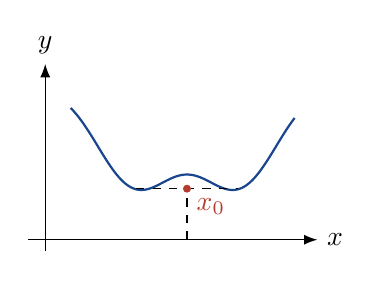
\begin{tikzpicture}[scale=0.72,>=Latex]
  \draw[->] (-0.3,0) -- (4.8,0) node[right] {$x$};
  \draw[->] (0,-0.2) -- (0,3.1) node[above] {$y$};
  \draw[thick,MainBlue,domain=0.45:4.4,smooth,samples=80]
    plot(\x,{0.28*(\x-2.5)^2+0.9+0.25*sin(180*\x)});
  \draw[dashed] (2.5,0) -- (2.5,0.9);
  \draw[dashed] (1.6,0.9) -- (3.4,0.9);
  \fill[AccentRed] (2.5,0.9) circle (2pt) node[below right] {$x_0$};
\end{tikzpicture}
\end{center}
\end{column}
\end{columns}
\end{frame}

\begin{frame}[t]{Fermat 定理的注记}
\small
\begin{enumerate}
  \item 若 $x_0$ 不是区间内点，则导数不必为零。例如 $f(x)=x$ 在 $[0,1]$ 的端点取得最值。
  \item 函数可在不可导点取极值。例如 $f(x)=|x|$ 在 $x=0$ 处取最小值，但不可导。
  \item 满足
  \[
    f'(x_0)=0
  \]
  的点称为驻点或临界点。驻点不一定是极值点，例如 $f(x)=x^3$ 的 $x=0$。
\end{enumerate}
\end{frame}

\begin{frame}[t]{定理 2：Darboux 定理}
\small
\begin{block}{结论}
设 $f$ 为 $[a,b]$ 上的可导函数，则 $f'$ 可以取到 $f'_+(a)$ 与 $f'_-(b)$ 之间的任意值。
\end{block}

设 $k$ 介于 $f'_+(a)$ 与 $f'_-(b)$ 之间。考虑
\[
  g(x)=f(x)-kx.
\]
则
\[
  g'_+(a)g'_-(b)=(f'_+(a)-k)(f'_-(b)-k)\le0.
\]
若等号成立，结论直接得到；若小于零，则 $g$ 在区间内部取到极值，由 Fermat 定理得到某个 $\xi\in(a,b)$ 使
\[
  g'(\xi)=0,\qquad f'(\xi)=k.
\]
\begin{alertblock}{结论理解}
导函数虽然未必连续，但它的值域仍具有介值性。
\end{alertblock}
\end{frame}

\begin{frame}[t]{例 30：闭区间上的最值}
\footnotesize
\[
  f(x)=x^3-x+1,\qquad x\in[-1,1].
\]
先求驻点：
\[
  f'(x)=3x^2-1=0,\qquad x=\pm\frac1{\sqrt3}.
\]
可能取最值的点为
\[
  -1,\quad -\frac1{\sqrt3},\quad \frac1{\sqrt3},\quad 1.
\]
计算函数值：
\[
  f(-1)=1,\qquad
  f\left(-\frac1{\sqrt3}\right)=1+\frac2{3\sqrt3},
\]
\[
  f\left(\frac1{\sqrt3}\right)=1-\frac2{3\sqrt3},\qquad
  f(1)=1.
\]
故最大值为
\[
  1+\frac2{3\sqrt3},
\]
最小值为
\[
  1-\frac2{3\sqrt3}.
\]
\end{frame}

\begin{frame}[t]{例 31：驻点不必是最值点}
\small
\[
  f(x)=x^3-x^2+1,\qquad x\in[-1,2].
\]
驻点由
\[
  f'(x)=3x^2-2x=x(3x-2)=0
\]
给出：
\[
  x=0,\qquad x=\frac23.
\]
候选点为
\[
  -1,\quad 0,\quad \frac23,\quad 2.
\]
函数值为
\[
  f(-1)=-1,\qquad f(0)=1,\qquad
  f\left(\frac23\right)=\frac{23}{27},\qquad f(2)=5.
\]
因此最小值为 $-1$，最大值为 $5$。
\end{frame}

\begin{frame}[t]{命题 2：非闭区间上的最值存在}
\small
\begin{block}{结论}
设 $f:\R\to\R$ 连续，且
\[
  \lim_{x\to-\infty}f(x)=\lim_{x\to+\infty}f(x)=+\infty.
\]
则 $f$ 在 $\R$ 上达到最小值。
\end{block}

证明思路：
\begin{enumerate}
  \item 取 $M>0$，使得 $|x|\ge M$ 时
  \[
    f(x)>f(0)+1.
  \]
  \item $f$ 在闭区间 $[-M,M]$ 上取到最小值，设为 $f(x_0)$。
  \item 由于 $0\in[-M,M]$，有 $f(x_0)\le f(0)$。
  \item 区间外 $f(x)>f(0)+1>f(x_0)$，所以 $x_0$ 也是整个 $\R$ 上的最小值点。
\end{enumerate}
\end{frame}

\begin{frame}[t]{例 32：平方距离和最小}
\small
设 $a_i,\ i=1,\ldots,n$ 为 $\R$ 上的 $n$ 个点，求一点 $x$，使得到这些点的距离平方和最小。

考虑
\[
  f(x)=\sum_{i=1}^n(x-a_i)^2.
\]
当 $|x|\to+\infty$ 时，$f(x)\to+\infty$，故最小值点存在。

由 Fermat 定理，最小值点满足
\[
  f'(x)=2\sum_{i=1}^n(x-a_i)=0.
\]
解得
\[
  \boxed{x=\frac1n\sum_{i=1}^n a_i.}
\]
也就是这些点的平均值。
\end{frame}

\begin{frame}[t]{例 33：Young 不等式}
\footnotesize
设 $p>1$，研究
\[
  f(x)=x-\frac{x^p}{p},\qquad x\in[0,+\infty).
\]
有
\[
  f'(x)=1-x^{p-1}.
\]
唯一驻点为 $x=1$，且它是最大值点：
\[
  f(x)\le f(1)=1-\frac1p,\qquad x\ge0.
\]
令
\[
  q=\frac{p}{p-1},
\]
上式等价于
\[
  x\le\frac{x^p}{p}+\frac1q.
\]
对 $a,b>0$，代入 $x=ab^{-1/(p-1)}$，整理得
\[
  \boxed{ab\le\frac{a^p}{p}+\frac{b^q}{q}.}
\]
等号成立当且仅当 $a^p=b^q$。
\end{frame}

\begin{frame}[t]{例 34：光线折射原理}
\small
\begin{columns}[T,onlytextwidth]
\begin{column}{0.55\textwidth}
两种介质中的光速分别为 $v_1,v_2$。光从
\[
  A=(0,a)
\]
经 $x$ 轴上一点 $(x,0)$ 到达
\[
  C=(b,-c).
\]
时间函数为
\[
  f(x)=\frac1{v_1}\sqrt{a^2+x^2}
      +\frac1{v_2}\sqrt{c^2+(b-x)^2}.
\]
极小点满足
\[
  \frac1{v_1}\frac{x}{\sqrt{a^2+x^2}}
  =
  \frac1{v_2}\frac{b-x}{\sqrt{c^2+(b-x)^2}}.
\]
\end{column}
\begin{column}{0.42\textwidth}
\begin{center}
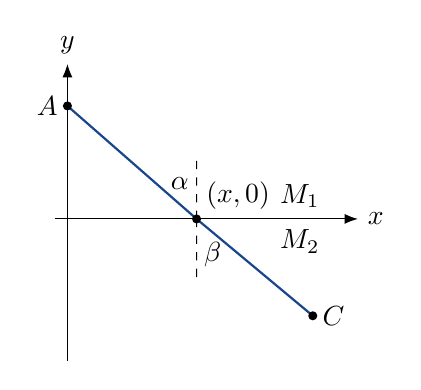
\begin{tikzpicture}[scale=0.82,>=Latex]
  \draw[->] (-0.2,0)--(4.5,0) node[right] {$x$};
  \draw[->] (0,-2.2)--(0,2.4) node[above] {$y$};
  \coordinate (A) at (0,1.75);
  \coordinate (P) at (2.0,0);
  \coordinate (C) at (3.8,-1.5);
  \draw[thick,MainBlue] (A)--(P)--(C);
  \fill (A) circle (2pt) node[left] {$A$};
  \fill (P) circle (2pt) node[above right] {$(x,0)$};
  \fill (C) circle (2pt) node[right] {$C$};
  \draw[dashed] (P)--(2,1.0);
  \draw[dashed] (P)--(2,-1.0);
  \draw (1.74,0.55) node {$\alpha$};
  \draw (2.25,-0.55) node {$\beta$};
  \node at (3.6,0.35) {$M_1$};
  \node at (3.6,-0.35) {$M_2$};
\end{tikzpicture}
\end{center}
\end{column}
\end{columns}

\[
  \boxed{\frac{\sin\alpha}{v_1}=\frac{\sin\beta}{v_2}}
  \qquad\text{或}\qquad
  \boxed{\frac{\sin\alpha}{\sin\beta}=\frac{v_1}{v_2}.}
\]
\end{frame}

\begin{frame}[t]{习题 16：题目}
\small
求下列函数的极值：
\[
  f_1(x)=2x^3-x^4,\qquad
  f_2(x)=x^2-3x+2,\qquad
  f_3(x)=x+\frac1x.
\]
\end{frame}

\begin{frame}[t]{习题 16：解答}
\footnotesize
\[
  f_1'(x)=2x^2(3-2x).
\]
$x=0$ 处导数不变号，不是极值点；$x=\frac32$ 处由正变负，故取极大值
\[
  f_1\left(\frac32\right)=\frac{27}{16}.
\]
\[
  f_2'(x)=2x-3,
\]
故 $x=\frac32$ 处取极小值
\[
  f_2\left(\frac32\right)=-\frac14.
\]
\[
  f_3'(x)=1-\frac1{x^2}.
\]
在 $x=-1$ 处取极大值 $-2$，在 $x=1$ 处取极小值 $2$。
\end{frame}

\begin{frame}[t]{习题 17：题目}
\small
求给定区间上的最大值和最小值：
\[
  f(x)=x^4(1-x),\quad x\in[0,1],
\]
\[
  g(x)=x^4-2x^2+5,\quad x\in[-2,2].
\]
\end{frame}

\begin{frame}[t]{习题 17：解答}
\small
对 $f$，
\[
  f'(x)=x^3(4-5x).
\]
候选点为 $0,\frac45,1$，函数值为
\[
  f(0)=0,\quad f(1)=0,\quad
  f\left(\frac45\right)=\frac{256}{3125}.
\]
故最小值为 $0$，最大值为 $\frac{256}{3125}$。

对 $g$，
\[
  g'(x)=4x(x^2-1).
\]
检查 $x=-2,-1,0,1,2$，得最小值 $4$，在 $x=\pm1$ 取得；最大值 $13$，在 $x=\pm2$ 取得。
\end{frame}

\begin{frame}[t]{习题 18：题目}
\small
求函数
\[
  f(x)=\sin^3x+\cos^3x
\]
的极值。
\end{frame}

\begin{frame}[t]{习题 18：解答}
\small
令
\[
  y=\sin x+\cos x,\qquad y\in[-\sqrt2,\sqrt2].
\]
由于
\[
  \sin^3x+\cos^3x
  =(\sin x+\cos x)(1-\sin x\cos x)
  =\frac{3y-y^3}{2},
\]
记 $h(y)=\frac{3y-y^3}{2}$。则
\[
  h'(y)=\frac32(1-y^2).
\]
因此主要极值为
\[
  \max f=1,\qquad \min f=-1.
\]
其中最大值在 $x=2k\pi$ 或 $x=\frac\pi2+2k\pi$ 取得；最小值在 $x=(2k+1)\pi$ 或 $x=\frac{3\pi}{2}+2k\pi$ 取得。
\end{frame}

\begin{frame}[t]{习题 19：题目}
\small
求函数
\[
  f(x)=x^3\ee^{-x}
\]
的极值。
\end{frame}

\begin{frame}[t]{习题 19：解答}
\small
求导得
\[
  f'(x)=\ee^{-x}x^2(3-x).
\]
临界点为 $x=0,3$。

在 $x=0$ 两侧，$f'(x)$ 均为正，故 $x=0$ 不是极值点。
在 $x=3$ 处，$f'(x)$ 由正变负，因此 $x=3$ 是极大值点，极大值为
\[
\boxed{f(3)=\frac{27}{\ee^3}.}
\]
\end{frame}

\begin{frame}[t]{习题 20：题目}
\small
求函数
\[
  f(x)=\frac{\ln x}{x},\qquad x>0
\]
的极值。
\end{frame}

\begin{frame}[t]{习题 20：解答}
\small
求导得
\[
  f'(x)=\frac{1-\ln x}{x^2}.
\]
因此唯一临界点为
\[
  x=\ee.
\]
当 $0<x<\ee$ 时，$f'(x)>0$；当 $x>\ee$ 时，$f'(x)<0$。
故 $x=\ee$ 处取极大值
\[
\boxed{f(\ee)=\frac1\ee.}
\]
该函数在 $(0,+\infty)$ 上无极小值。
\end{frame}

\begin{frame}[t]{习题 21：题目}
\small
给出光线反射定律的极值证明。

设光线从 $A=(a,h)$ 经 $x$ 轴上一点 $P=(x,0)$ 反射到 $B=(b,k)$，其中 $h,k>0$。证明最短路径满足入射角等于反射角。
\end{frame}

\begin{frame}[t]{习题 21：解答}
\small
路径长度为
\[
  L(x)=\sqrt{(x-a)^2+h^2}+\sqrt{(x-b)^2+k^2}.
\]
极小点满足
\[
  L'(x)=
  \frac{x-a}{\sqrt{(x-a)^2+h^2}}
  +\frac{x-b}{\sqrt{(x-b)^2+k^2}}=0.
\]
即
\[
  \frac{x-a}{|AP|}
  =
  \frac{b-x}{|PB|}.
\]
左、右两边分别为入射角与反射角的正弦，因此两角相等。
\end{frame}

\begin{frame}[t]{习题 22：题目}
\small
设 $p\ge1$，证明 Bernoulli 不等式：
\[
  (1+x)^p\ge1+px,\qquad x\ge-1.
\]
\end{frame}

\begin{frame}[t]{习题 22：解答}
\small
令
\[
  F(x)=(1+x)^p-1-px,\qquad x\ge-1.
\]
则
\[
  F(0)=0,\qquad
  F'(x)=p\bigl((1+x)^{p-1}-1\bigr).
\]
当 $x\ge0$ 时，$F'(x)\ge0$，故 $F(x)\ge F(0)=0$。

当 $-1\le x\le0$ 时，$F'(x)\le0$，因此 $F$ 在 $[-1,0]$ 上递减，仍有
\[
  F(x)\ge F(0)=0.
\]
所以
\[
  (1+x)^p\ge1+px.
\]
\end{frame}

\begin{frame}[t]{习题 23：题目}
\small
设 $f$ 在 $[a,b]$ 上可导，并且
\[
  f'(a)<\lambda<f'(b).
\]
利用极值思想证明：存在 $\xi\in(a,b)$，使得
\[
  f'(\xi)=\lambda.
\]
\end{frame}

\begin{frame}[t]{习题 23：解答}
\small
令
\[
  F(x)=f(x)-\lambda x.
\]
则
\[
  F'(a)=f'(a)-\lambda<0,\qquad
  F'(b)=f'(b)-\lambda>0.
\]
由 $F'(a)<0$，$F$ 在 $a$ 右侧先下降；由 $F'(b)>0$，$F$ 在 $b$ 左侧随 $x$ 增大而上升。
因此 $F$ 的最小值不能只在端点取得，必在某个内点 $\xi\in(a,b)$ 取得。

由 Fermat 定理，
\[
  F'(\xi)=0.
\]
即
\[
\boxed{f'(\xi)=\lambda.}
\]
\end{frame}

\end{document}
